% L5c lecture companion: follows the current notebook's teaching sequence.
% Source notebook SHA-256:
% da1765266e40336abd9a37bbbef8c18f51383bbde2c92e6b13e3fe44fa0ef6fc
% The style files and Cornell seal are copied unchanged from L5a/slides.
% Both mathematical figures are vector conversions of the lecture's SVGs.
% Setup stays in the notebook, following the supplied reference decks.
\documentclass[aspectratio=169,11pt]{beamer}
\usepackage{vnslides}
\usepackage{tabularx}

\renewcommand{\vnlecturecode}{L5c}
\newcolumntype{Y}{>{\raggedright\arraybackslash}X}
\newcommand{\lecturelink}{https://github.com/varnerlab/CHEME-5800-CourseRepository-Fall-2026/blob/main/weeks/week-05/L5c/CHEME-5800-L5c-Lecture-LinearProgramming-Fall-2026.ipynb}
\newcommand{\examplelink}{https://github.com/varnerlab/CHEME-5800-CourseRepository-Fall-2026/blob/main/weeks/week-05/L5c/CHEME-5800-L5c-FruitProblem-Primal-Example-Fall-2026.ipynb}
\newcommand{\kktlink}{https://github.com/varnerlab/CHEME-5800-CourseRepository-Fall-2026/blob/main/weeks/week-05/L5c/CHEME-5800-L5c-LagrangeKKT-Advanced-Fall-2026.ipynb}
\newcommand{\simplexlink}{https://github.com/varnerlab/CHEME-5800-CourseRepository-Fall-2026/blob/main/weeks/week-05/L5c/CHEME-5800-L5c-RevisedSimplex-Algorithm-Fall-2026.ipynb}
\newcommand{\interiorlink}{https://github.com/varnerlab/CHEME-5800-CourseRepository-Fall-2026/blob/main/weeks/week-05/L5c/CHEME-5800-L5c-InteriorPointMethod-Algorithm-Fall-2026.ipynb}
\newcommand{\lablink}{https://github.com/varnerlab/CHEME-5800-CourseRepository-Fall-2026/blob/main/weeks/week-05/L5d/CHEME-5800-L5d-Lab-MinimumCostAssignmentFlow-Fall-2026.ipynb}
\newcommand{\cutlablink}{https://github.com/varnerlab/CHEME-5800-CourseRepository-Fall-2026/blob/main/weeks/week-05/L5b/CHEME-5800-L5b-Lab-MaximumFlowSensitivity-Fall-2026.ipynb}
\newcommand{\ecolilink}{https://arxiv.org/abs/2607.07677}
\newcommand{\lecturesource}[1]{\note{[Sources]\par
  \href{\lecturelink}{L5c lecture: Introduction to Linear Programming.}\par
  #1\par[/Sources]}}

\title{\texorpdfstring{{\vnheavy L5c}}{L5c}: Introduction to Linear Programming}
\subtitle{\texorpdfstring{Allocation, duality, and resource values\\[3pt]CHEME 5800 Cornell University}{Allocation, duality, and resource values; CHEME 5800 Cornell University}}
\author{Copyright Jeffrey Varner 2026. All Rights Reserved}

\begin{document}
\special{pdf:minorversion 7}

\vntitlepage

% Notebook: introduction and three learning objectives.
\begin{frame}{Objectives for Today}
  How should we allocate limited resources among competing uses, and how can
  we show that a feasible allocation is optimal?

  \vspace{0.35em}
  {\large\textbf{\ink{Today's concepts}}}
  \vspace{0.2em}
  \begin{itemize}\setlength{\itemsep}{0.55em}
    \item \hilite{Formulate resource-allocation models}: identify decision
      variables, objective coefficients, constraints, and bounds in
      consumer-choice and minimum-cost-flow problems.
    \item \hilite{Explain duality and resource values}: construct the dual,
      show how feasible dual solutions bound the primal objective, and read
      the optimal dual variable as the value of an extra dollar of budget.
    \item \hilite{Evaluate optimization results}: distinguish feasible from
      optimal; check status, recompute the objective, and verify constraints
      and bounds.
  \end{itemize}

  \slidenote{Lecture:}{\href{\lecturelink}{Introduction to Linear Programming}}
  \lecturesource{Introduction and Learning Objectives.}
\end{frame}

% Notebook: Examples; setup stays in the example notebook.
\begin{frame}{Lecture and Example}
  \textbf{\ink{Lecture:}}
  \href{\lecturelink}{Introduction to Linear Programming}

  Formulate consumer-choice and network-flow models as linear programs, then
  use duality to bound the objective and interpret the value of a resource.

  \vspace{1.2em}
  \textbf{\ink{Example:}}
  \href{\examplelink}{Two Goods Resource Allocation Problem: Apples versus Oranges}

  Formulate the primal program that maximizes utility within a budget,
  predict the purchase from utility per dollar, and solve it with the
  course package.

  \vspace{0.8em}
  Optional notebooks on solver algorithms are collected near the end.
  \lecturesource{Examples and the linked apples-versus-oranges example notebook.}
\end{frame}

% Notebook: Primal Linear Programming Problems.
\begin{frame}{Primal Linear Programming Problems}
  Suppose a \hilite{linear} objective of the continuous decision vector
  $\mathbf x\in\mathbb R^n$ is constrained by $m$ linear inequalities.
  The \hilite{primal} linear program is:
  \[
    \begin{aligned}
      \text{minimize/maximize}\quad
        & \sum_{i=1}^n c_i x_i\\
      \text{subject to}\quad & \mathbf A\mathbf x\leq\mathbf b,
        \qquad\mathbf A\in\mathbb R^{m\times n},\ \mathbf b\in\mathbb R^m,\\
        & x_i\geq0,\qquad i=1,2,\ldots,n.
    \end{aligned}
  \]

  \vspace{0.3em}
  \begin{itemize}\setlength{\itemsep}{0.55em}
    \item $c_i\in\mathbb R$: objective coefficients; $x_i\in\mathbb R$: decision variables.
    \item $\mathbf A$ and $\mathbf b$: the constraint matrix and right-hand side vector.
  \end{itemize}

  \vspace{0.4em}
  The goal is to minimize or maximize the objective while satisfying the constraints.
  \lecturesource{Primal Linear Programming Problems: general form.}
\end{frame}

\begin{frame}{What Does It Mean to Solve This Model?}
  A decision vector is \hilite{feasible} if it satisfies every constraint and
  bound. All feasible vectors form the \hilite{feasible region}.

  \vspace{0.7em}
  \begin{itemize}\setlength{\itemsep}{0.65em}
    \item An \hilite{optimal} vector $\mathbf x^\star$ is feasible and attains
      the best objective value over that region: the largest for a
      maximization, the smallest for a minimization.
    \item A feasible vector need not be optimal, and several different vectors
      can attain the same optimal value.
    \item If no feasible vector exists, the model is \hilite{infeasible}.
    \item If feasible vectors give arbitrarily good objective values, the
      problem is \hilite{unbounded} and has no finite optimum.
  \end{itemize}

  \vspace{0.6em}
  These outcomes depend on the objective, constraints, and bounds together.
  \lecturesource{Primal Linear Programming Problems: feasibility, optimality, infeasibility, and unboundedness.}
\end{frame}

% Notebook: Consumer Choice Problems as Linear Programs.
\begin{frame}{Consumer Choice as a Linear Program}
  Let there be $n$ products. For product $i$, let $u_i$ be its utility score
  and $p_i$ its price per unit. The consumer has a budget $I$ and buys
  $x_i$ units of product $i$, so total cost is $\sum_i p_i x_i$ and
  utility is $U(x_1,\ldots,x_n)=\sum_i u_i x_i$.

  \vspace{0.3em}
  The consumer maximizes utility while staying within the budget:
  \[
    \begin{aligned}
      \text{maximize}\quad
        & \sum_{i=1}^n u_i x_i\\
      \text{subject to}\quad & \sum_{i=1}^n p_i x_i\leq I,\\
        & x_i\geq0,\qquad i=1,2,\ldots,n.
    \end{aligned}
  \]
  The optimal solution, if it exists, gives the number of units of each
  product to purchase. Production planning, transportation, and network flow
  can be formulated in the same way.
  \lecturesource{Consumer Choice Problems as Linear Programs.}
\end{frame}

% Example notebook: data cell, bounds, and utility per dollar (Case A).
\begin{frame}{Case A: Apples versus Oranges}
  Let $x_1$ and $x_2$ be the quantities of apples and oranges.
  Apples cost 2 dollars per unit and give 0.55 utility units;
  oranges cost 4 dollars per unit and give 0.45 utility units.
  The budget is 100 dollars:
  \[
    \begin{aligned}
      \underset{x_1,x_2}{\text{maximize}}\quad
        & U(x_1,x_2)=0.55x_1+0.45x_2\\
      \text{subject to}\quad & 2x_1+4x_2\leq100,\qquad x_1,x_2\geq0.
    \end{aligned}
  \]
  Spending the whole budget on one fruit sets a finite upper bound
  $x_i\leq I/p_i$: at most \hilite{50 apples} or \hilite{25 oranges}.

  \vspace{0.4em}
  Utility per dollar decides which fruit we buy:
  \[
    \frac{u_1}{p_1}=\frac{0.55}{2}=\hilite{0.275},
    \qquad
    \frac{u_2}{p_2}=\frac{0.45}{4}=0.1125.
  \]
  Apples win, so the optimum is $(x_1^\star,x_2^\star)=(50,0)$ with $U^\star=27.5$.
  \lecturesource{Example notebook: Constants and Problem Data; bounds from the budget; What should we expect?
    \href{\examplelink}{Apples versus Oranges example.}}
\end{frame}

% Example notebook: three utility settings in the data cell.
\begin{frame}{Three Utility Settings, Three Solution Cases}
  Keep prices $(p_1,p_2)=(2,4)$ and budget $I=100$ fixed.
  The data cell offers three utility settings:

  \vspace{0.7em}
  \renewcommand{\arraystretch}{1.45}
  \setlength{\tabcolsep}{5pt}
  \begin{tabularx}{\textwidth}{@{}lccYr@{}}
    \toprule
    Case & $(u_1,u_2)$ & $(u_1/p_1,u_2/p_2)$ & Optimal purchase & Utility\\
    \midrule
    A & $(0.55,0.45)$ & $(0.275,0.1125)$ & $(50,0)$, apples only & 27.5\\
    B & $(0.15,0.55)$ & $(0.075,0.1375)$ & $(0,25)$, oranges only & 13.75\\
    C & $(2,4)$ & $(1,1)$ & Any full-budget mix & 100\\
    \bottomrule
  \end{tabularx}

  \vspace{0.9em}
  The fruit we buy depends on utility \hilite{per dollar}, not on utility
  alone. With linear utility we typically get a \hilite{corner solution}.

  \vspace{0.5em}
  In the special Case C the ratios are equal, so every mixture that spends the
  full budget is optimal: infinitely many solutions share the same utility.
  \lecturesource{Example notebook: data cell cases A, B, C and What should we expect?}
\end{frame}

\begin{frame}{The Optimum Is a Corner or an Entire Edge}
  \begin{center}
    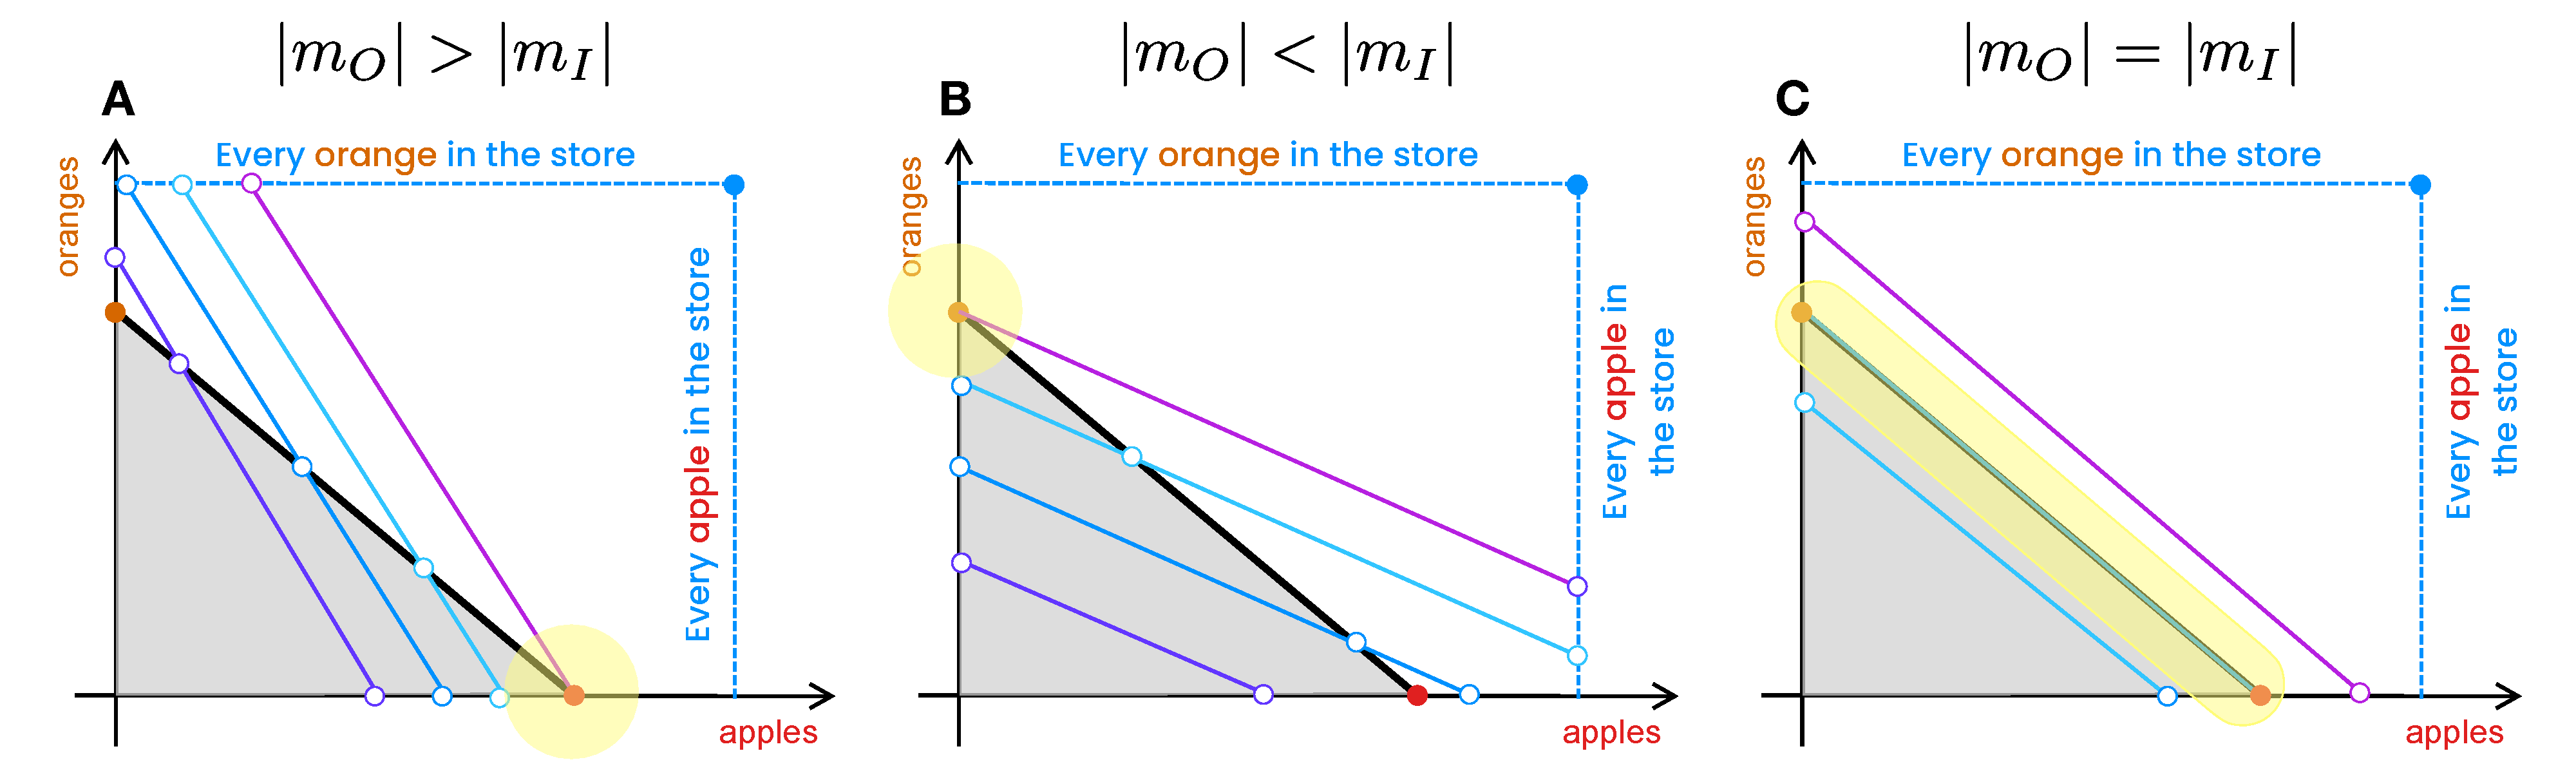
\includegraphics[width=0.86\textwidth]{assets/Fig-ThreeCases-LP-Schematic.pdf}
  \end{center}
  \vspace{-0.25em}
  Compare the slope of the budget line, $m_I=-p_1/p_2$, with the slope of a
  line of constant utility, $m_O=-u_1/u_2$:
  \begin{itemize}\setlength{\itemsep}{0.3em}
    \item \textbf{\ink{Case A:}} $|m_I|<|m_O|$ gives the apple corner.
    \item \textbf{\ink{Case B:}} $|m_I|>|m_O|$ gives the orange corner.
    \item \textbf{\ink{Case C:}} $|m_I|=|m_O|$ makes the whole budget edge optimal.
  \end{itemize}
  \lecturesource{Example notebook: What should we expect? Three solution cases.
    Schematic: ../figs/Fig-ThreeCases-LP-Schematic.svg; provenance in ../figs/README.md.}
\end{frame}

% Notebook: Does E. coli have free will?
\begin{frame}{Does \emph{E.~coli} Have Free Will?}
  A bacterium must allocate its limited proteome among competing enzymes
  to maximize growth. This is a consumer-choice problem:

  \vspace{0.6em}
  \begin{itemize}\setlength{\itemsep}{0.65em}
    \item \hilite{Budget:} the total protein the cell can devote to enzymes.
    \item \hilite{Products:} the sugars it can metabolize; each enzyme returns
      growth per unit of protein invested.
    \item \hilite{Objective:} maximize growth rate within the proteome budget.
  \end{itemize}

  \vspace{0.6em}
  Because the utility is linear, the optimum is a \hilite{corner}: the cell
  commits its budget to the single most profitable sugar and consumes sugars
  in sequence. Only equally profitable sugars are used together, along the
  budget line.

  \slidenote{Reading:}{\href{\ecolilink}{Rethinking the Choice Behavior of Sugar Metabolism in Bacteria (arXiv)}}
  \lecturesource{Consumer Choice Problems: Does E. coli have free will? Linked arXiv paper.}
\end{frame}

% Notebook: Minimum Cost Network Flow Problems as Linear Programs.
\begin{frame}{Minimum-Cost Network Flow}
  A directed graph $G=(\mathcal V,\mathcal E)$ has source, sink, and
  intermediate nodes. Edges carry goods or resources between nodes.

  \vspace{0.7em}
  \begin{itemize}\setlength{\itemsep}{0.65em}
    \item Each edge $j\in\mathcal E$ has a capacity $c_j$, the most flow
      it can carry, and a cost $w_j$ per unit of flow.
    \item $f_j$ is the flow on edge $j$; $s$ is the source and $t$ the sink.
    \item The goal: deliver a specified amount of flow from $s$ to $t$ at
      \hilite{minimum total cost}.
  \end{itemize}

  \vspace{0.6em}
  Several routings can deliver the same amount; their costs differ.
  \lecturesource{Minimum Cost Network Flow Problems as Linear Programs: formulation box.}
\end{frame}

\begin{frame}{An Incidence Matrix Encodes the Graph}
  The matrix $\mathbf A\in\mathbb R^{|\mathcal V|\times|\mathcal E|}$
  has one row per node $i$ and one column per edge $j$.
  Its entries and the right-hand side $b_i$ are:

  \vspace{0.5em}
  \begin{columns}[T,onlytextwidth]
    \begin{column}{0.55\textwidth}
      \[
        A_{ij}=\begin{cases}
          1,&\text{edge }j\text{ is incoming to }i,\\
          -1,&\text{edge }j\text{ is outgoing from }i,\\
          0,&\text{otherwise}.
        \end{cases}
      \]
    \end{column}
    \begin{column}{0.41\textwidth}
      \[
        b_i=\begin{cases}
          -F,&i=s\ \text{(source)},\\
          F,&i=t\ \text{(sink)},\\
          0,&\text{otherwise}.
        \end{cases}
      \]
    \end{column}
  \end{columns}

  \vspace{0.7em}
  Here $F$ is the total flow from source to sink. The source generates flow,
  the sink consumes it, and every other node conserves it:
  \[
    \underbrace{(\mathbf A\mathbf f)_i}_{\text{inflow minus outflow}}=b_i.
  \]
  \lecturesource{Incidence matrix convention and right-hand side vector.}
\end{frame}

\begin{frame}{The Minimum-Cost Flow Linear Program}
  Collect the edge flows in $\mathbf f\in\mathbb R^{|\mathcal E|}$ and the
  net inflows in $\mathbf b\in\mathbb R^{|\mathcal V|}$:
  \[
    \begin{aligned}
      \text{minimize}\quad
        & \sum_{j\in\mathcal E} w_j f_j\\
      \text{subject to}\quad & \mathbf A\mathbf f=\mathbf b,\\
        & 0\leq f_j\leq c_j,\qquad\forall j\in\mathcal E.
    \end{aligned}
  \]

  \vspace{0.6em}
  \begin{itemize}\setlength{\itemsep}{0.7em}
    \item The objective adds the cost incurred on every edge.
    \item The equalities enforce the required delivery and flow conservation.
    \item The bounds keep every edge flow nonnegative and within capacity.
  \end{itemize}
  The optimal solution, if it exists, is the cheapest routing that delivers $F$.
  \lecturesource{Minimum cost flow as a primal linear program.}
\end{frame}

% Notebook: Worked Network: Choosing Between Two Routes.
\begin{frame}{Worked Network: Two Routes}
  Deliver $F=3$ flow units from $s$ to $t$. Edge labels give capacity in flow
  units and cost in dollars per flow unit.

  \vspace{0.2em}
  \begin{center}
    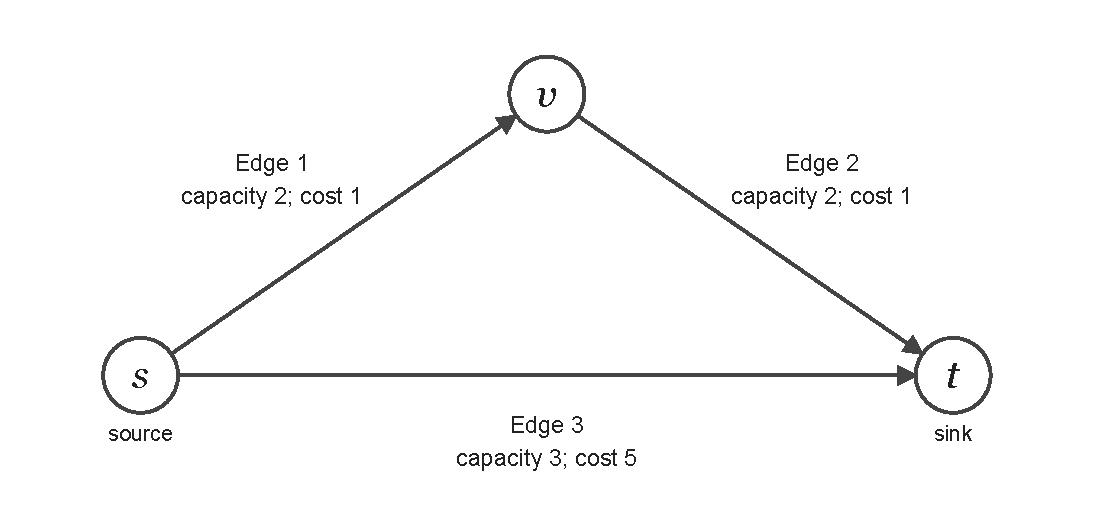
\includegraphics[width=0.56\textwidth]{assets/Fig-MinCostFlow-ThreeNode.pdf}
  \end{center}

  Through $v$: cost $1+1=2$ dollars per unit, but capacity 2.
  Direct edge 3: cost 5 dollars per unit.

  \vspace{0.6em}
  Some of the 3-unit delivery must travel over edge 3.
  \lecturesource{Worked Network: Choosing Between Two Routes.
    Diagram: ../figs/Fig-MinCostFlow-ThreeNode.svg; provenance in ../figs/README.md.}
\end{frame}

\begin{frame}{Write the Three Node Balances}
  Order rows as $(s,v,t)$ and columns as edges $(1,2,3)$.
  For $F=3$, the equality constraints $\mathbf A\mathbf f=\mathbf b$ are:
  \[
    \underbrace{\begin{bmatrix}-1&0&-1\\1&-1&0\\0&1&1\end{bmatrix}}_{\mathbf A}
    \underbrace{\begin{bmatrix}f_1\\f_2\\f_3\end{bmatrix}}_{\mathbf f}
    =\underbrace{\begin{bmatrix}-3\\0\\3\end{bmatrix}}_{\mathbf b}.
  \]

  \vspace{0.4em}
  \begin{itemize}\setlength{\itemsep}{0.6em}
    \item Source: $f_1+f_3=3$ units leave.
    \item Intermediate vertex: $f_1=f_2$.
    \item Sink: $f_2+f_3=3$ units enter.
  \end{itemize}
  Each edge column has a $-1$ where the edge begins and a $+1$ where it ends.
  \lecturesource{Worked network: ordered incidence matrix and node balances.}
\end{frame}

\begin{frame}{The Program With the Numbers Filled In}
  With costs $\mathbf w=(1,1,5)$ and capacities $\mathbf c=(2,2,3)$,
  the primal linear program for this network is:
  \[
    \begin{aligned}
      \text{minimize}\quad & f_1+f_2+5f_3\\
      \text{subject to}\quad & f_1+f_3=3,\\
        & f_1-f_2=0,\\
        & f_2+f_3=3,\\
        & 0\leq f_1\leq2,\quad 0\leq f_2\leq2,\quad 0\leq f_3\leq3.
    \end{aligned}
  \]

  \vspace{0.4em}
  This is the general model with numbers substituted: the objective is
  $\sum_j w_j f_j$, the three equalities are the rows of
  $\mathbf A\mathbf f=\mathbf b$, and the bounds are $0\leq f_j\leq c_j$.
  \lecturesource{Worked network: the primal program with numbers substituted.}
\end{frame}

\begin{frame}{Solve by Hand: Fill the Cheaper Route First}
  The equalities leave one free variable. Let $q$ be the flow along the
  route through $v$: $f_1=f_2=q$ and $f_3=3-q$, with $0\leq q\leq2$
  from the bounds on edges 1 and 2.

  \vspace{0.4em}
  Substitute into the total cost:
  \[
    C(q)=\sum_{j\in\mathcal E}w_j f_j
        =(1)(q)+(1)(q)+(5)(3-q)=15-3q.
  \]
  Cost decreases with $q$, so use the full capacity of the cheaper route:
  \[
    (f_1^\star,f_2^\star,f_3^\star)=(2,2,1),
    \qquad C^\star=\hilite{9}\text{ dollars}.
  \]
  Sending all 3 units directly over edge 3 is feasible but costs 15 dollars.
  Conservation and capacity checks establish feasibility; the cost comparison
  selects the preferred routing.
  \lecturesource{Worked network: one-variable cost reduction and optimal flow.}
\end{frame}

\begin{frame}{What Does This Small Example Tell Us?}
  \begin{itemize}\setlength{\itemsep}{0.6em}
    \item \hilite{The solver does the search.} A solver searches the feasible
      set defined by the constraints and bounds for the point that minimizes
      the objective. Here that set was a line segment, so we searched by hand;
      larger networks need a solver.
    \item \hilite{The required flow is data, not a decision.} Asking for more
      than the network can carry, here more than the 5 units that can leave
      the source, makes the linear program infeasible.
    \item \hilite{The same formulation scales.} The
      \href{\lablink}{L5d lab} uses this incidence convention for a
      worker–task assignment model and examines what changes when an
      assignment becomes unavailable.
  \end{itemize}

  \vspace{0.5em}
  Formulating the model is our job; finding the best point in the feasible
  set is the solver's.
  \lecturesource{Worked network: closing bullets and the L5d connection.}
\end{frame}

% Notebook: Dual Linear Programming Problems; What Is the Consumer's Budget Worth?
\begin{frame}{Dual Linear Programming Problems}
  The primal returns a purchase. How do we know that no other feasible
  purchase does better?

  \vspace{0.5em}
  In the \href{\cutlablink}{L5b lab}, a cut answered this question for flows:
  every feasible flow had to cross the cut, so the cut capacity bounded every
  flow. We want a similar check for a linear program.

  \vspace{0.7em}
  \textbf{\ink{The idea: put a price on the budget.}}
  Let $y\geq0$ be the value of one dollar of budget, in utility units per dollar.
  Product $i$ costs $p_i$ dollars and delivers $u_i$ utility units, so it
  returns $u_i/p_i$ utility per dollar.

  \vspace{0.5em}
  If $y$ is at least the return of every product, so that
  $p_i y\geq u_i$ for all $i$, then no way of spending $I$ dollars can earn
  more than \hilite{$Iy$} utility units.
  \lecturesource{What Is the Consumer's Budget Worth? The idea of pricing the budget.}
\end{frame}

\begin{frame}{Why Does This Give a Bound?}
  Take any feasible purchase $\mathbf x\geq\mathbf 0$ and any $y\geq0$
  with $p_i y\geq u_i$ for every product. Replace each utility by the larger
  quantity $p_i y$, then use the budget constraint:
  \[
    U(\mathbf x)=\sum_{i=1}^n u_i x_i
    \leq\sum_{i=1}^n(p_i y)\,x_i
    =y\sum_{i=1}^n p_i x_i
    \leq yI.
  \]

  \vspace{0.6em}
  \begin{itemize}\setlength{\itemsep}{0.8em}
    \item First inequality: $u_i\leq p_i y$ and $x_i\geq0$.
    \item Last inequality: $\sum_i p_i x_i\leq I$ and $y\geq0$.
  \end{itemize}

  \vspace{0.7em}
  Any such $y$ gives an upper bound: no feasible purchase earns more than
  $Iy$ utility units.
  \lecturesource{What Is the Consumer's Budget Worth? Why does this give a bound?}
\end{frame}

\begin{frame}{The Dual Finds the Smallest Upper Bound}
  Different valid values of $y$ give different bounds; the smallest is the
  most informative. Minimizing $Iy$ over valid $y$ is the
  \hilite{consumer dual problem}:
  \[
    \begin{aligned}
      \underset{y}{\text{minimize}}\quad & Iy\\
      \text{subject to}\quad & p_i y\geq u_i,\qquad i=1,\ldots,n,\\
        & y\geq0.
    \end{aligned}
  \]
  The constraints say $y\geq u_i/p_i$ for every product, so the smallest
  feasible $y$ is the best return available:
  \[
    y^\star=\max_i\frac{u_i}{p_i},
  \]
  the product with the \hilite{biggest bang for the buck}.
  The optimal dual value $Iy^\star$ is the best upper bound on utility, and
  any feasible purchase that attains it is optimal.
  \lecturesource{What Is the Consumer's Budget Worth? The consumer dual problem.}
\end{frame}

\begin{frame}{What Is the Consumer's Budget Worth?}
  Take Case A: apples cost 2 dollars and give 0.55 utility units per unit,
  oranges cost 4 dollars and give 0.45, and $I=100$ dollars.
  The dual constraints are $2y\geq0.55$ and $4y\geq0.45$, so:
  \[
    y^\star=\max\!\left\{\frac{0.55}{2},\frac{0.45}{4}\right\}=0.275,
    \qquad Iy^\star=27.5.
  \]

  \vspace{0.5em}
  Buying 50 apples and no oranges is feasible (it spends exactly 100 dollars)
  and attains $0.55\cdot50=27.5$ utility units.

  \vspace{0.5em}
  That equals the dual bound $Iy^\star=27.5$, so no feasible purchase can do
  better: this purchase is \hilite{optimal}.
  \lecturesource{Consumer dual example for Case A: matching bound.}
\end{frame}

\begin{frame}{Both Inequalities Hold With Equality}
  Substitute $\mathbf x=(50,0)$ and $y^\star=0.275$ into the chain:
  \[
    \begin{aligned}
      \underbrace{0.55\cdot50+0.45\cdot0}_{U(\mathbf x)=27.5}
      &\;\leq\;
      \underbrace{(2\cdot0.275)\cdot50+(4\cdot0.275)\cdot0}_{=27.5}\\[10pt]
      &\;=\;
      \underbrace{0.275\cdot(2\cdot50+4\cdot0)}_{=27.5}
      \;\leq\;
      \underbrace{0.275\cdot100}_{Iy^\star=27.5}.
    \end{aligned}
  \]

  \vspace{0.4em}
  The first holds with equality because every unit bought (apples) has
  $p_i y^\star=u_i$ exactly; the second because the purchase spends the whole budget.

  \vspace{0.7em}
  \textbf{\ink{Shadow price.}} $y^\star=0.275$ is the budget's
  \hilite{shadow price} in utility units per dollar: an additional dollar buys
  0.5 units of apples and increases optimal utility by 0.275.

  \slidenote{Assumes:}{fixed prices and utilities, divisible quantities, and sufficient availability. In general models, shadow prices can change as resource availability changes.}
  \lecturesource{Consumer dual example: equality in the chain and the shadow price.}
\end{frame}

% Notebook: The General Primal-Dual Pair.
\begin{frame}{The General Primal–Dual Pair}
  \begin{columns}[T,onlytextwidth]
    \begin{column}{0.47\textwidth}
      \textbf{\ink{Primal problem}}
      \[
        \begin{aligned}
          \text{maximize}\ \, & \sum_{i=1}^n c_i x_i\\
          \text{s.t.}\ \, & \sum_{i=1}^n A_{j,i}x_i\leq b_j,\ \ j=1,\ldots,m,\\
            & x_i\geq0,\ \ i=1,\ldots,n.
        \end{aligned}
      \]
    \end{column}
    \begin{column}{0.50\textwidth}
      \textbf{\ink{Dual problem}}
      \[
        \begin{aligned}
          \text{minimize}\ \, & \sum_{j=1}^m b_j y_j\\
          \text{s.t.}\ \, & \sum_{j=1}^m A_{j,i}y_j\geq c_i,\ \ i=1,\ldots,n,\\
            & y_j\geq0,\ \ j=1,\ldots,m.
        \end{aligned}
      \]
    \end{column}
  \end{columns}

  \vspace{0.9em}
  The consumer problem is this pair with a single constraint, $m=1$:
  the coefficients $c_i$ are the utilities $u_i$, the one constraint row
  $A_{1,i}$ holds the prices $p_i$, the right-hand side $b_1$ is the budget
  $I$, and the lone dual variable $y_1$ is the budget value $y$.
  \lecturesource{The General Primal-Dual Pair.}
\end{frame}

% Notebook: What has changed?
\begin{frame}{What Has Changed Between Primal and Dual?}
  With $\mathbf A\in\mathbb R^{m\times n}$, $\mathbf c\in\mathbb R^n$,
  and $\mathbf b\in\mathbb R^m$ as above:

  \vspace{0.5em}
  \begin{enumerate}\setlength{\itemsep}{0.6em}
    \item The \hilite{sense of the objective flips}: a maximization primal has
      a minimization dual. A minimization primal with
      $\mathbf A\mathbf x\geq\mathbf b$, $\mathbf x\geq\mathbf 0$ has the
      maximization dual $\mathbf A^\top\mathbf y\leq\mathbf c$, $\mathbf y\geq\mathbf 0$.
    \item Primal objective coefficients $c_i$ become the dual right-hand side.
    \item Primal right-hand side constants $b_j$ become the dual objective coefficients.
    \item The constraint matrix is \hilite{transposed}:
      $\sum_{j=1}^m A_{j,i}y_j$ is component $i$ of $\mathbf A^\top\mathbf y$.
    \item Variables and constraints \hilite{swap counts}: the primal has $n$
      variables and $m$ constraints; the dual has $m$ variables and $n$ constraints.
  \end{enumerate}
  \lecturesource{What has changed? Items 1 through 5.}
\end{frame}

\begin{frame}{Constraints and Variables Are Paired, With Signs}
  Each primal constraint $j$ gives a dual variable $y_j$, and each primal
  variable $x_i$ gives a dual constraint $i$:

  \vspace{0.6em}
  \renewcommand{\arraystretch}{1.45}
  \begin{tabularx}{\textwidth}{@{}YY@{}}
    \toprule
    Primal condition & Corresponding dual condition\\
    \midrule
    $\sum_i A_{j,i}x_i\leq b_j$ & $y_j\geq0$\\
    $\sum_i A_{j,i}x_i=b_j$ & $y_j$ free (no sign restriction)\\
    $x_i\geq0$ & $\sum_j A_{j,i}y_j\geq c_i$\\
    $x_i$ free & $\sum_j A_{j,i}y_j=c_i$\\
    \bottomrule
  \end{tabularx}

  \vspace{0.8em}
  The network-flow model uses equality balances $\mathbf A\mathbf f=\mathbf b$,
  so its dual variables are free.
  \lecturesource{What has changed? Item 6: pairing of constraints and variables with signs.}
\end{frame}

\begin{frame}{Weak and Strong Duality}
  For the maximization primal and its dual:
  \[
    \max\{\mathbf c^\top\mathbf x:\mathbf A\mathbf x\leq\mathbf b,\ \mathbf x\geq\mathbf 0\}
    \qquad\text{and}\qquad
    \min\{\mathbf b^\top\mathbf y:\mathbf A^\top\mathbf y\geq\mathbf c,\ \mathbf y\geq\mathbf 0\}.
  \]

  \vspace{0.3em}
  \begin{itemize}\setlength{\itemsep}{0.8em}
    \item \hilite{Weak duality.} For any primal-feasible $\mathbf x$ and
      dual-feasible $\mathbf y$,
      $\mathbf c^\top\mathbf x\leq\mathbf b^\top\mathbf y$.
      The primal optimum is bounded above by the dual optimum; the difference
      is the \hilite{duality gap}.
    \item \hilite{Strong duality.} If both problems are feasible with finite
      optimal values, then
      $\max\{\mathbf c^\top\mathbf x\}=\min\{\mathbf b^\top\mathbf y\}$,
      so the duality gap is zero.
  \end{itemize}

  \vspace{0.6em}
  A feasible primal candidate whose objective matches a feasible dual bound
  is optimal, as the 50-apple purchase was.
  \lecturesource{Duality: weak and strong duality bullets.}
\end{frame}

% Notebook: How a Solver Fits the Modeling Workflow.
\begin{frame}{How a Solver Fits the Modeling Workflow}
  We supply variables, an objective, constraints, and bounds; the solver
  reports why it stopped and, when available, a candidate. Before interpreting it:

  \vspace{0.3em}
  \begin{enumerate}\setlength{\itemsep}{0.45em}
    \item \hilite{Read the status.} An optimal status means optimal within
      numerical tolerances. A time or iteration limit may leave a feasible
      candidate without proving optimality; an infeasible or unbounded model
      has no finite optimum.
    \item \hilite{Verify feasibility.} Substitute into the original constraints
      and bounds: expenditure versus budget, or every node balance in
      $\mathbf A\mathbf f=\mathbf b$ and every edge bound.
    \item \hilite{Recompute the objective.} Use the returned quantities and the
      original coefficients; compare with the reported value.
    \item \hilite{Check an optimality bound.} Verify dual feasibility, then
      compare $\mathbf b^\top\mathbf y$ with $\mathbf c^\top\mathbf x$.
      A zero gap proves optimality in exact arithmetic.
  \end{enumerate}

  \slidenote{Tolerances:}{account for the units and scales of the quantities compared. See the \href{https://jump.dev/JuMP.jl/stable/manual/solutions/}{JuMP solution guide}.}
  \lecturesource{How a Solver Fits the Modeling Workflow. External documentation:
    \url{https://jump.dev/JuMP.jl/stable/manual/solutions/}.}
\end{frame}

% Notebook: Optional Advanced Material and Lab Exercises.
\begin{frame}{Optional: How a Solver Finds an Optimum}
  Three optional notebooks, not prerequisites for the L5d lab, read in order:

  \vspace{0.7em}
  \begin{itemize}\setlength{\itemsep}{0.7em}
    \item \href{\kktlink}{\hilite{Lagrange multipliers and KKT conditions}.}
      Why can't we just use Lagrange multipliers on a linear program? Adding
      multipliers for the nonnegativity bounds gives the Karush–Kuhn–Tucker
      conditions, necessary and sufficient for optimality.
    \item \href{\simplexlink}{\hilite{Revised simplex}.} How does a solver move
      from one corner to a better one? Basic and nonbasic variables, reduced
      costs, and the ratio test.
    \item \href{\interiorlink}{\hilite{Interior-point methods}.} What if we
      cross the interior instead of walking the edges? A logarithmic barrier,
      perturbed KKT residuals, and Newton steps.
  \end{itemize}

  \slidenote{Lab L5d:}{\href{\lablink}{formulate and solve a worker–task minimum-cost flow with JuMP and GLPK.}}
  \lecturesource{Optional Advanced Material and Lab Exercises.}
\end{frame}

% Notebook: Summary; preserve three retrospective takeaways.
\begin{frame}{Summary}
  We developed linear programs for consumer choice and network flow, then
  used duality to bound the objective and value a limited resource.

  \vspace{0.3em}
  {\large\textbf{\ink{Key takeaways}}}
  \vspace{0.2em}
  \begin{itemize}\setlength{\itemsep}{0.5em}
    \item \textbf{\ink{Formulating allocation models.}} We expressed purchases
      and flows using continuous variables, linear objectives, and resource or
      balance constraints.
    \item \textbf{\ink{Interpreting duality and resource values.}} We used
      feasible dual solutions to bound the primal objective and read optimal
      dual variables as shadow prices, the marginal value of a resource.
    \item \textbf{\ink{Evaluating optimization results.}} We distinguished
      feasibility from optimality, checked status, constraints, bounds, and a
      recomputed objective, and proved optimality by matching primal and dual values.
  \end{itemize}

  \vspace{0.4em}
  The primal asks how best to use the resources; the dual bounds what they
  can achieve. Reaching that bound justifies optimality.
  \lecturesource{Summary; takeaways remain independent of numerical example values.}
\end{frame}

\end{document}
